\section{抛物线}

本节要点:
\begin{itemize}
    \item 掌握抛物线的概念;
    \item 从代数角度掌握抛物线的几何性质。
\end{itemize}

%============================================================
\subsection{抛物线及其标准方程}

\begin{definition}[抛物线]
设二维平面中有两个定点$F$和直线$l$,设它们距离为$p>0$,若平面上的点和$F,l$的距离相等,则称这些点组成的集合为{\bf 抛物线},常用$P$表示,若令$F=\left( \frac{p}{2},0 \right) ,l:x=-\frac{p}{2}$,则抛物线可以表示为下列的{\bf 标准方程}:
\[
y=2px \quad p>0
\]
其中,$F$称为{\bf 焦点},$l$称为{\bf 准线}。
\end{definition}

\begin{figure}[h]
\centering
\begin{tikzpicture}[line join=round, scale=0.3]
\pgfmathparse{0.6/0.3}
\mydrawxy{-7}{7}{-5}{5}
\draw[thick,domain=0:5,samples=200] plot (\x,{ sqrt(4*(\x))}); % p=2
\draw[thick,domain=0:5,samples=200] plot (\x,{-sqrt(4*(\x))});
\coordinate[label=below left:{$O$}] (O) at (0,0);
\coordinate[label=below:     {$F$}] (F) at (1,0);
\coordinate[                      ] (K) at (-1,0);
\coordinate[label=above:     {$M$}] (M) at (4,4);
\draw[thick] (-1,5)--(-1,-5);
\draw (-1,4)--(M)--(F);
\fill (F) circle (\pgfmathresult mm);
\coordinate[label=above:{$p$}] (p) at ($(O)+(0,0.5)$);
\draw[decorate,decoration={calligraphic brace,raise=0cm,aspect=0.5,amplitude=0.2cm},thick] (K)--(F);
\end{tikzpicture}
\end{figure}

\begin{tcolorbox}
详细阅读课本关于双曲线标准方程的推导过程,体会两次平方的意义。详细阅读例2、例4、例5。
\end{tcolorbox}

%============================================================
\subsection{抛物线的简单几何性质}

我们称:
\begin{itemize}
    \item $y=0$:{\bf 轴};
    \item $\left( 0,0 \right) $:{\bf 顶点};
    \item $e=1$:{\bf 离心率},恒为1。
\end{itemize}

%============================================================
\subsection{拓展讨论:焦点}

从焦点出发的光线经抛物线反射成平行光,沿抛物线的轴入射的平行光汇聚于焦点,证明这点需要微积分的知识,略。

\begin{figure}[ht]
\centering
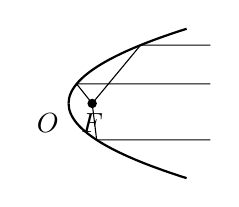
\begin{tikzpicture}[line join=round, scale=0.3]
\pgfmathparse{0.6/0.3}
\mydrawxy{-7}{7}{-4}{4}
\draw[thick,domain=0:5,samples=200] plot (\x,{ sqrt(2*(\x))});
\draw[thick,domain=0:5,samples=200] plot (\x,{-sqrt(2*(\x))});
\coordinate[label=below left:{$O$}] (O)  at (0,0);
\coordinate[label=below:     {$F$}] (F)  at (1,0);
\coordinate                         (P1) at (3.05,2.47);
\coordinate                         (P2) at (0.34,0.83);
\coordinate                         (P3) at (1.19,-1.54);
\fill (F) circle (\pgfmathresult mm);
\draw (F)--(P1)--(6,2.47);
\draw (F)--(P2)--(6,0.83);
\draw (F)--(P3)--(6,-1.54);
\end{tikzpicture}
\end{figure}

反射式望远镜就是由抛物面和双曲线构成,抛物面的焦点和双曲面的一个焦点重合。遥远的星体发出的光线可以认为是平行光,到达抛物面反射后汇聚于焦点,再由双曲面反射,形成的虚像位于双曲面的另一个焦点,这样,星体就像位于双曲面的另一个焦点一样,使得星体看起来更近了,详见教材本章小结的拓广探索15。

对于焦点,我们还可以这么思考。设有$F_1,F_2$两个焦点,若从$F_1$射出的光线经曲线反射汇聚于$F_2$,则曲线构成椭圆。当$F_2$逐渐远离$F_1$,椭圆变得越来越扁平,当$F_2$置于无穷远处时,光线经曲线反射称为平行线,此时椭圆变成了抛物线。对于离心率:
\[
\lim_{c\rightarrow a} e=\lim_{c\rightarrow a} \frac{c}{a}=1
\]

%============================================================
\subsection{拓展讨论:抛物线的一般方程}

采用极坐标的形式,抛物线绕顶点沿顺时针转$\alpha $后的方程如下:
\begin{align*}
&y^2=2px \\
&\left[ r\sin \left( \theta -\alpha \right) \right] ^2=2pr\cos \left( \theta -\alpha \right) \\
&\cos ^2\alpha \cdot y^2-\sin 2\alpha \cdot xy+\sin ^2\alpha \cdot x^2=2p\cos \alpha \cdot x+2p\sin \alpha \cdot y
\end{align*}
注意我们这里是顺时针转动图形,相当于逆时针转动坐标系,所以是$-\alpha $而不是$+\alpha $。对比椭圆和双曲线,不难发现,抛物线的特征是有关于$x,y$的一次项。




